\newpage
\section{Problem 5.19}
\subsection{重要数据展示}
求解对称正定的方程组$\bm{Gx}=\bm{b}$可以看作极小化二次函数\[q(\bm{x})=\dfrac{1}{2}\bm{x^TGx-b^Tx}\]
\[\bm{g}(\bm{x})=\nabla q(\bm{x})=\bm{Gx}-\bm{b}\]
其中,$\nabla^2 q(\bm{x})=\bm{G}$为Hilbert矩阵。

希尔伯特矩阵是一种系数都是单位分数的方块矩阵,希尔伯特矩阵$\bm{H}$的第$i$横行第$j$纵列的系数是$H_{{ij}}={\dfrac  {1}{i+j-1}}$

以5阶的Hilbert矩阵为例,其矩阵如下:
\[H_5=\left(\begin{array}{ccccc} 1 & \frac{1}{2} & \frac{1}{3} & \frac{1}{4} & \frac{1}{5}\\ \frac{1}{2} & \frac{1}{3} & \frac{1}{4} & \frac{1}{5} & \frac{1}{6}\\ \frac{1}{3} & \frac{1}{4} & \frac{1}{5} & \frac{1}{6} & \frac{1}{7}\\ \frac{1}{4} & \frac{1}{5} & \frac{1}{6} & \frac{1}{7} & \frac{1}{8}\\ \frac{1}{5} & \frac{1}{6} & \frac{1}{7} & \frac{1}{8} & \frac{1}{9} \end{array}\right)\]

希尔伯特矩阵是一种数学变换矩阵,正定,且高度病态(即,任何一个元素发生一点变动,整个矩阵的行列式的值和逆矩阵都会发生巨大变化),病态程度和阶数相关。

希尔伯特矩阵的一个特点就是条件数特别大,以上面的5阶Hilbert矩阵为例,当范数为$l_2$矩阵范数时,其条件数大约是$4.8\times 10^{5}$

经证明:当 $ n\rightarrow \infty$的时候,$ n\times n$的希尔伯特矩阵的条件数近似为$O((1+{\sqrt  {2}})^{{4n}}/{\sqrt  {n}})$

MATLAB中有直接生成$N$阶希尔伯特矩阵的函数:\boxed{hilb(N)}

\newpage
\subsection{算法伪代码}
\begin{algorithm}[h]  
\caption{Conjugate gradient method method for problem(5.19)}  
\begin{algorithmic}[1]  
\STATE Given $\bm{x}^{(0)}$  and $\bm{G}$
\STATE Set $\bm{g}^{(0)}=\bm{Gx}^{(0)}-\bm{b}$
\STATE Set $\bm{p}^{(0)}=-\bm{g}^{(0)},k=0$
\WHILE {$\|\bm{g}^{(k)}\|>\epsilon$}
\STATE Set $\bm{d}=\bm{G}\bm{p}^{(k)}$
\STATE Set $\alpha_k=\dfrac{{\bm{g}^{(k)}}^T\bm{g}^{(k)}}{{\bm{p}^{(k)}}^T\bm{d}}$
\STATE Set $\bm{x}^{(k+1)}=\bm{x}^{(k)}+\alpha_k\bm{p}^{(k)}$
\STATE Set $\bm{g}^{(k+1)}=\bm{g}^{(k)}+\alpha_k\bm{d}$
\STATE Set $\beta_{k+1}=\dfrac{{\bm{g}^{(k+1)}}^T\bm{g}^{(k+1)}}{{\bm{g}^{(k)}}^T{\bm{g}^{(k)}}}$
\STATE Set $\bm{p}^{(k+1)}=-\bm{g}^{(k+1)}+\beta_{k+1}\bm{p}^{(k)}$
\STATE Set $k=k+1$
\ENDWHILE
\RETURN $\bm{x}^{(k)}$ as $\bm{x}^{\star}$
\end{algorithmic}  
\end{algorithm}

\subsection{迭代结果展示}
求解不同阶数Hilbert矩阵的迭代次数列成表格如下:

\begin{table}[htbp]
  \centering
  \caption{迭代次数}
    \begin{tabular}{ccccc}
\toprule
\textbf{n} &5& 8& 12 & 20 \\
	\midrule
\textbf{step}&6   & 19  & 35  & 66 \\
\bottomrule
    \end{tabular}
\end{table}

\begin{figure}[H]
\centering
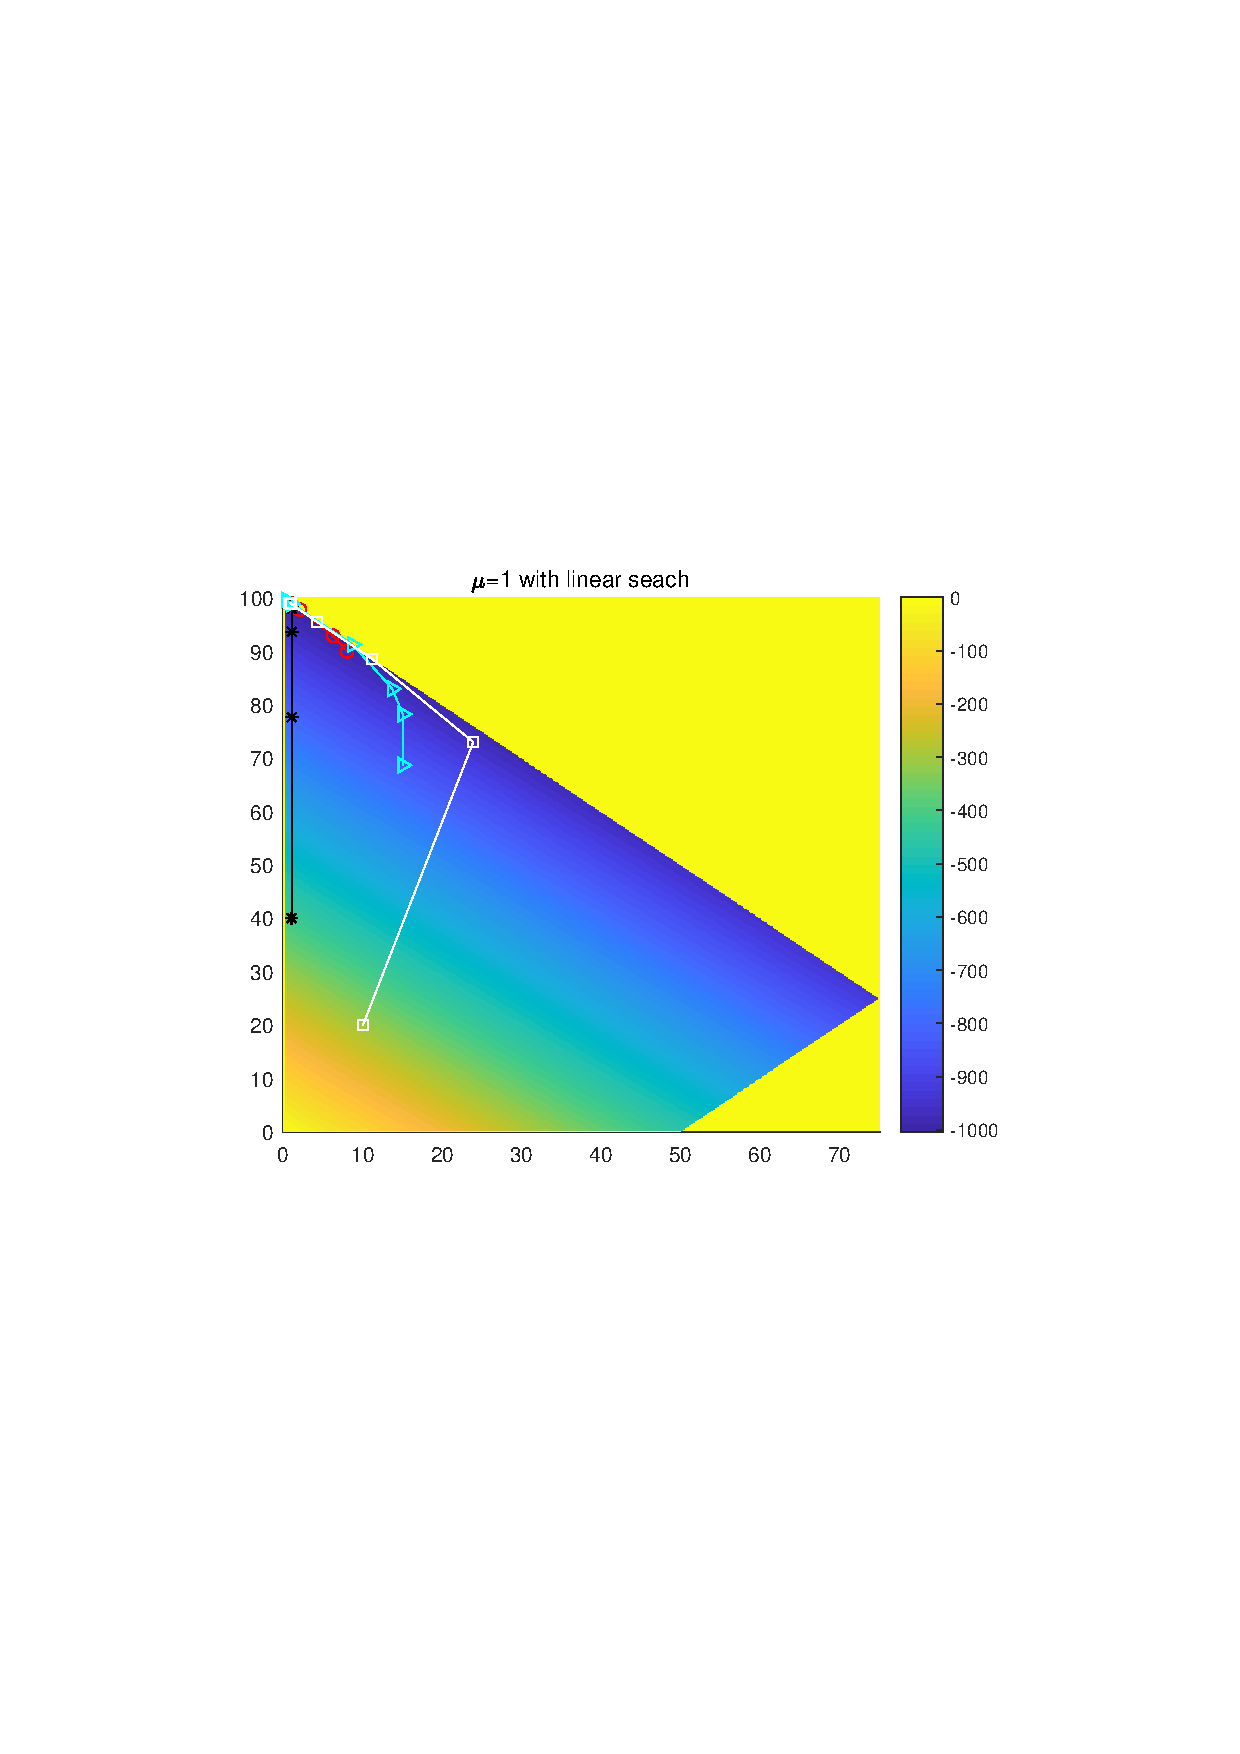
\includegraphics[width=10.5cm]{fig/5_1.pdf}
%\caption{5阶Hilbert矩阵}
\end{figure}

\begin{figure}[H]
\centering
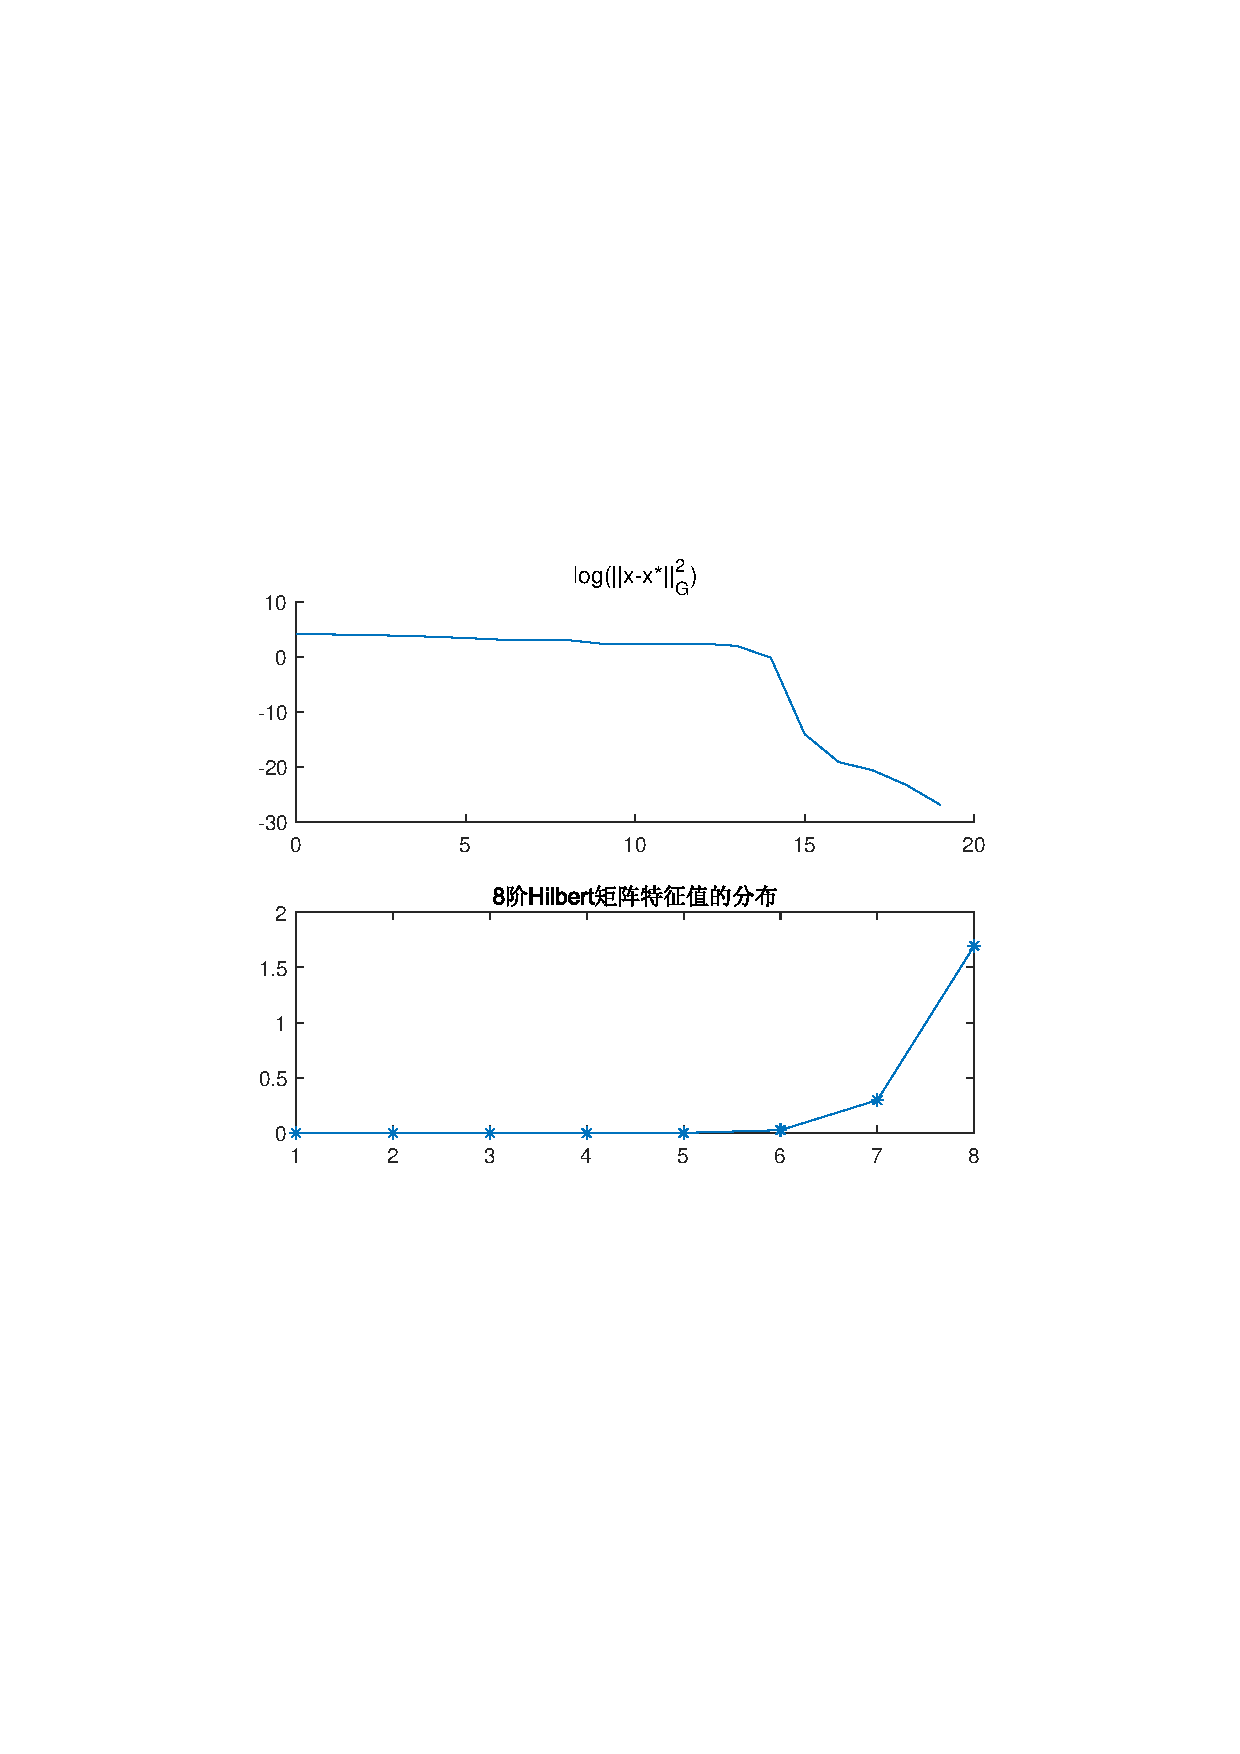
\includegraphics[width=10.5cm]{fig/5_2.pdf}
%\caption{8阶Hilbert矩阵}
\end{figure}

\begin{figure}[H]
\centering
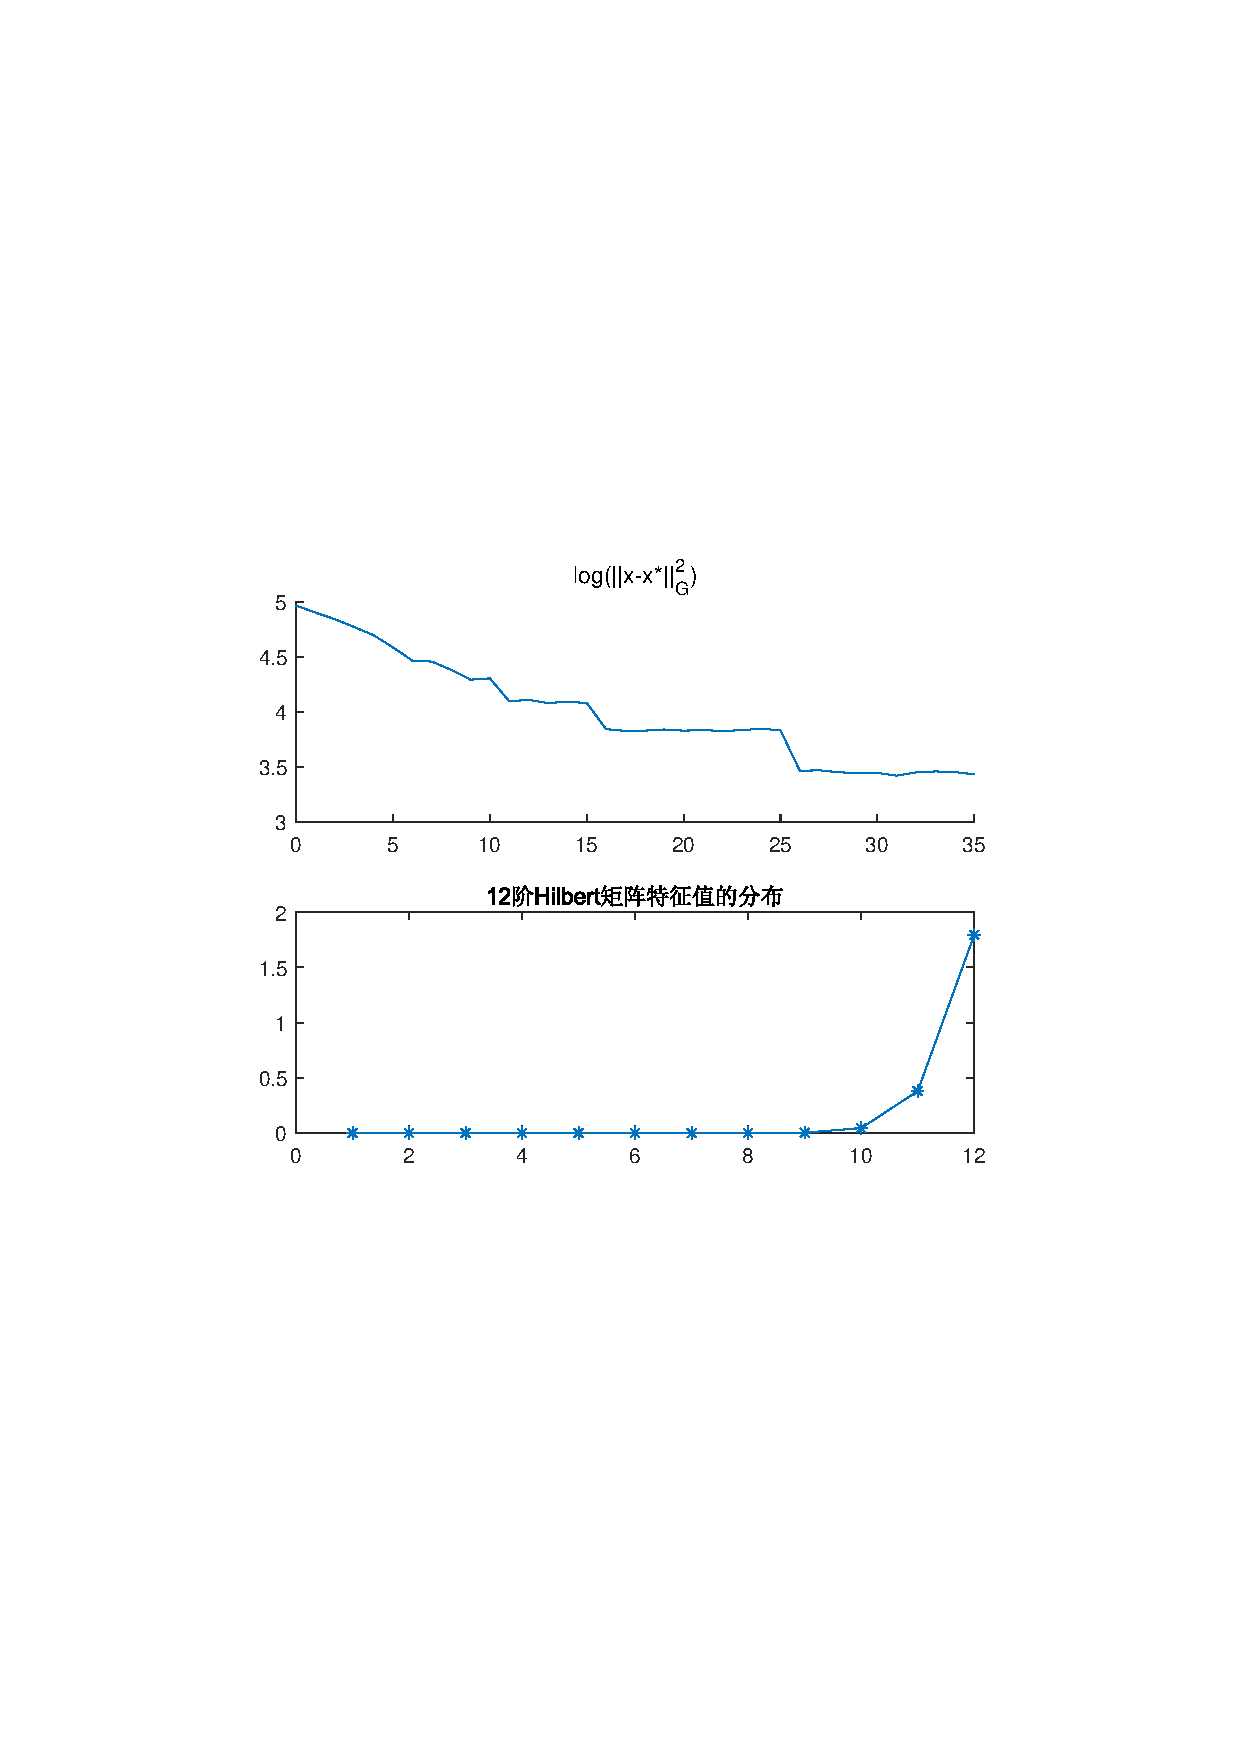
\includegraphics[width=10.5cm]{fig/5_3.pdf}%\caption{12阶Hilbert矩阵}
\end{figure}

\begin{figure}[H]
\centering
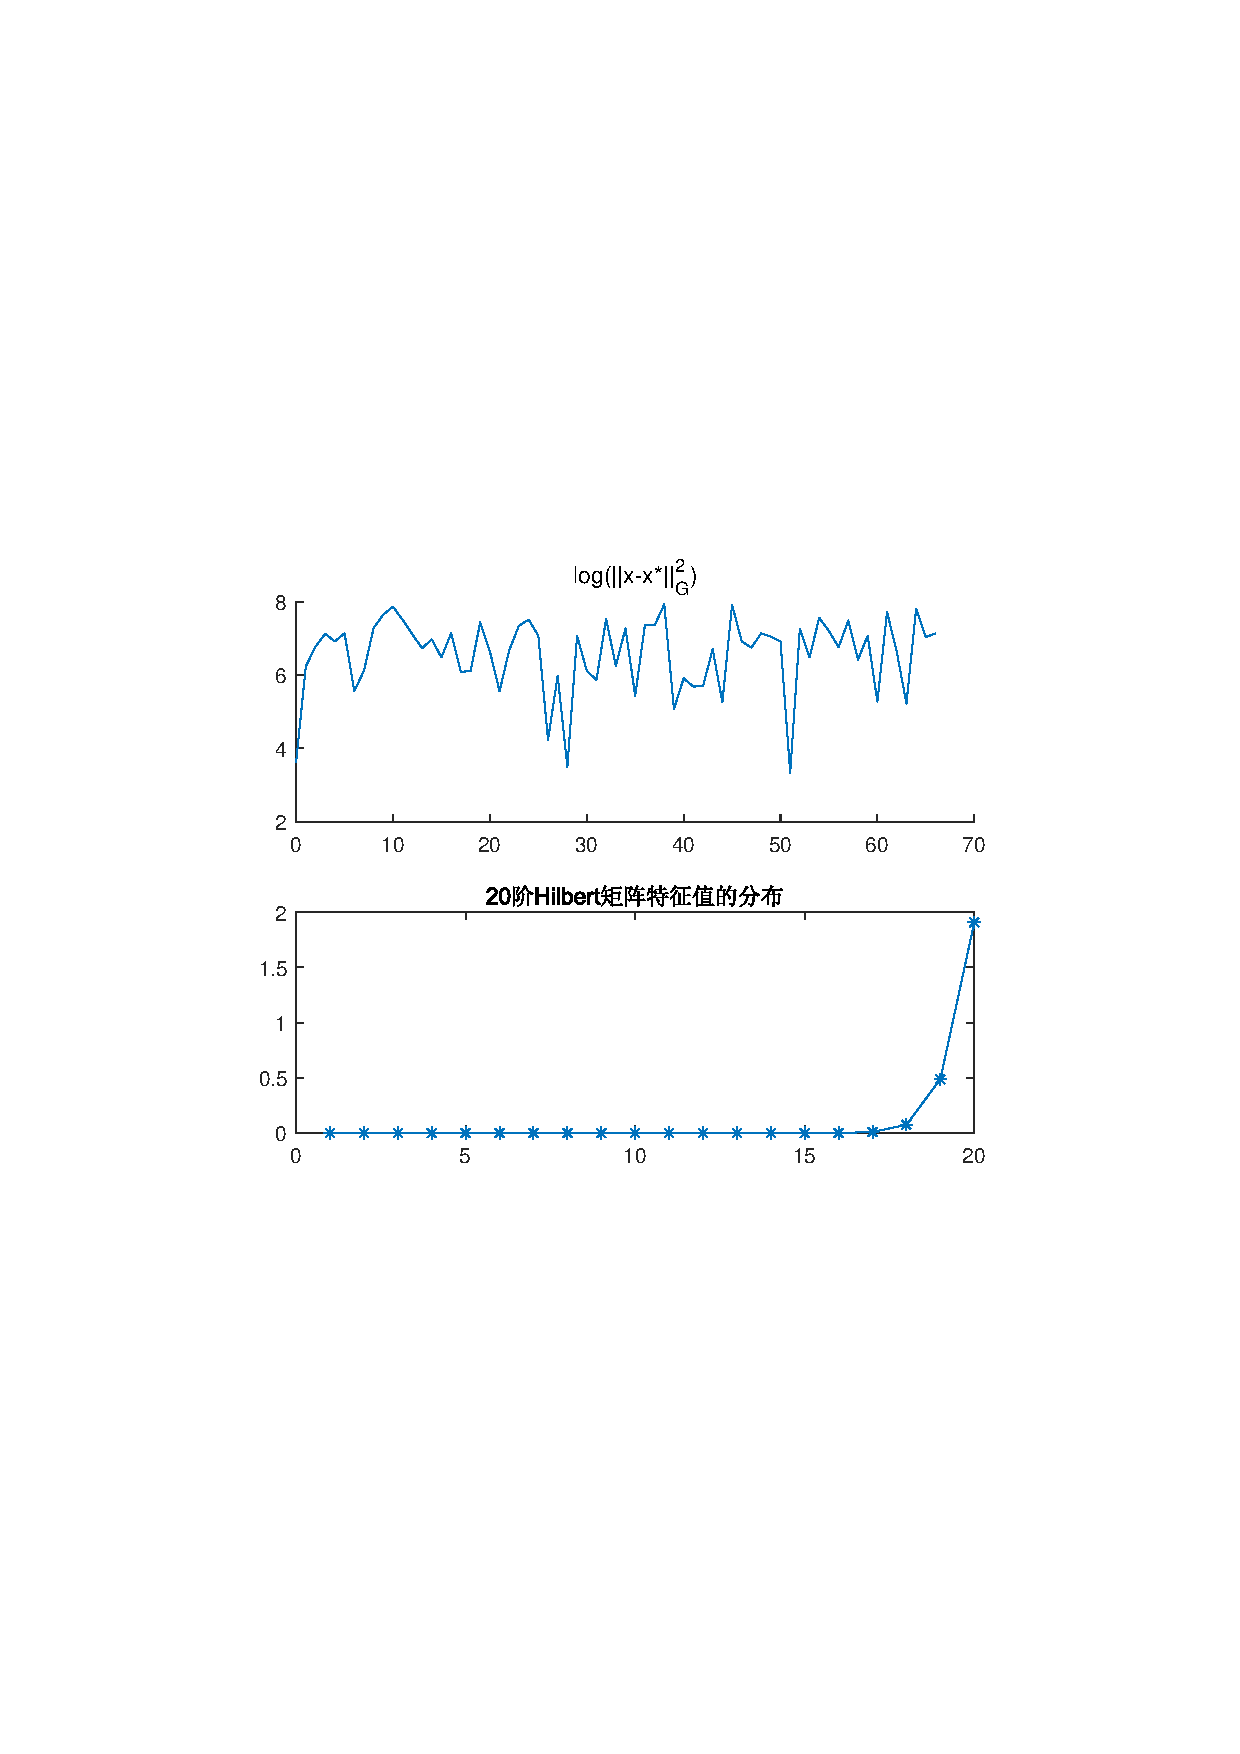
\includegraphics[width=10.5cm]{fig/5_4.pdf}
%\caption{20阶Hilbert矩阵}
\end{figure}

\subsection{总结分析}
首先我们通过一个小程序考察一下Hilbert矩阵的病态性质:

\begin{lstlisting}
N=20;
G=random('unif',0,1,[N N]);
G1=inv(G);
I=eye(N);
norm(G*G1-I)

%ans =
%
%  2.9348e-14
\end{lstlisting}

先生成一个$20\times 20$的随机矩阵,然后用MATLAB自带的求逆函数inv()求逆,然后将原矩阵与其逆相乘再减去单位阵,之后求矩阵范数,求得结果为2.9348e-14,可见MATLAB自带的求逆函数在面对一般问题时还是比较精确的。

\begin{lstlisting}
N=20;
H=hilb(N);
H_inv=inv(H);
I=eye(N);
norm(H*H_inv-I)

%ans =
%
%  33.8220
\end{lstlisting}



然后我们对Hilbert矩阵进行相同操作,结果为33.8220,远远大于上面那个结果,足以见Hilbert矩阵的高度病态性质。

另外,我们由书本知识可以知道:共轭梯度法与特征值的分布有关,当特征值分布较密集时,相同步数迭代精度更高。所以我们可以对Hilbert矩阵进行预处理,降低其条件数。

嗯,那如何对Hilbert矩阵进行预处理呢?我在网上经过不懈的搜索,终于在Alfi Quarteroni Fausto Saleri的 Scientifi Computing with MATLAB and Octave中找到这么一个题目(见图\ref{exam}),题目中点出可以用Hilbert矩阵对角元素构建一个对角矩阵,作为预处理矩阵。

\begin{figure}[H]
\centering
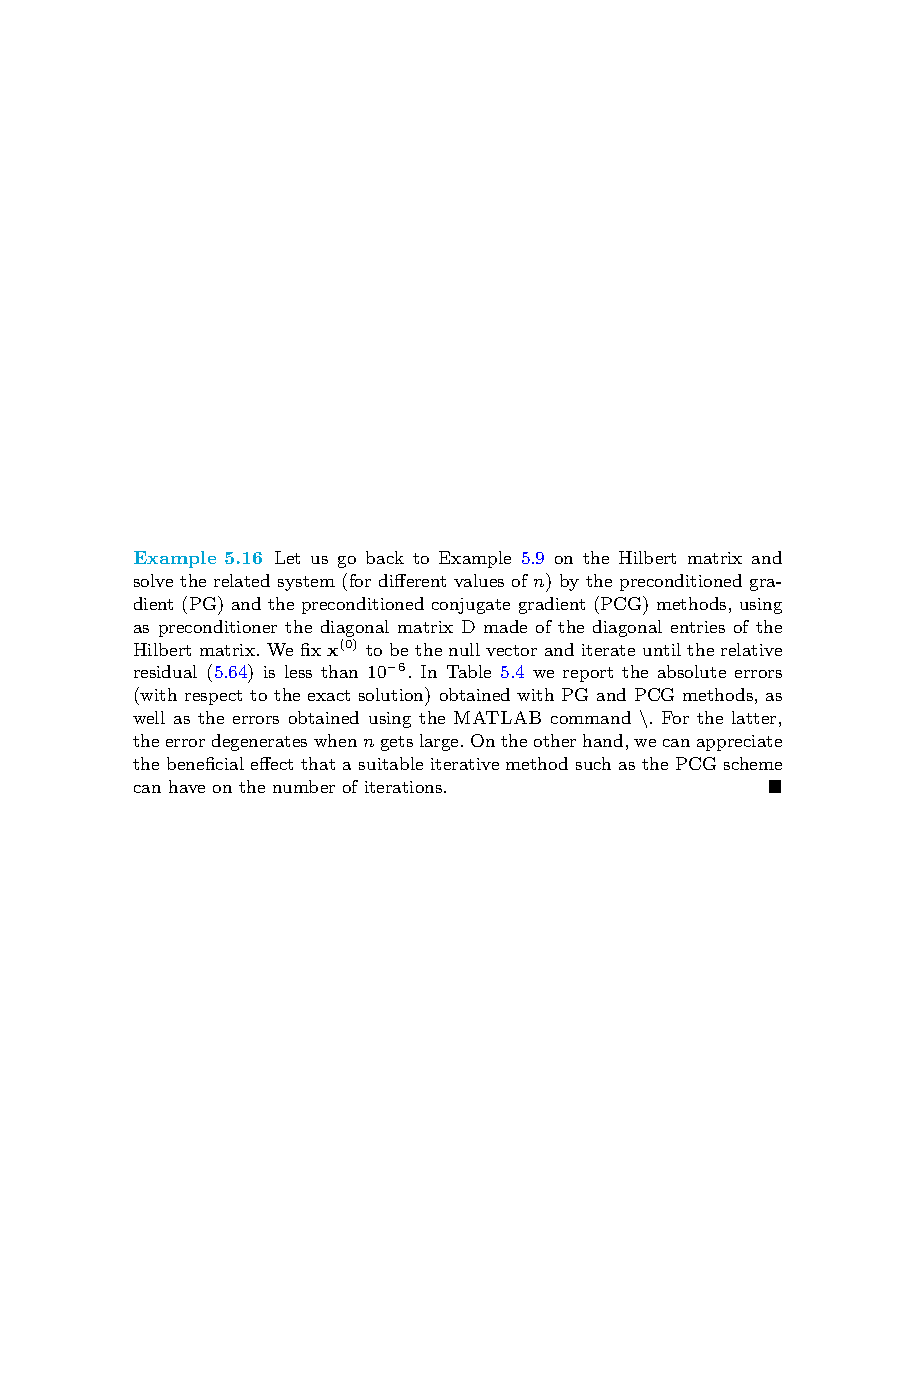
\includegraphics[width=12cm]{fig/5_5.pdf}
\caption{从书上摘的题}
\label{exam}
\end{figure}

也就是说,设$C$是由$G$的对角线元素开方构成的对角矩阵,令$\hat{G}=C^{-T}GC^{-1},\quad \hat{x}=Cx$,经过变换可调整为$M^{-1}Gx=M^{-1}b$,其中$M=C^TC$,即由$G$对角线元素构成的对角阵。

经过这么一番预处理后,不难看出不难看出该
矩阵仍然是对称正定矩阵,而且其对角元素全为 1.

那么我就使用书上的预处理共轭梯度法首先对$N=20$的Hilbert矩阵进行检验:

\begin{figure}[H]
\centering
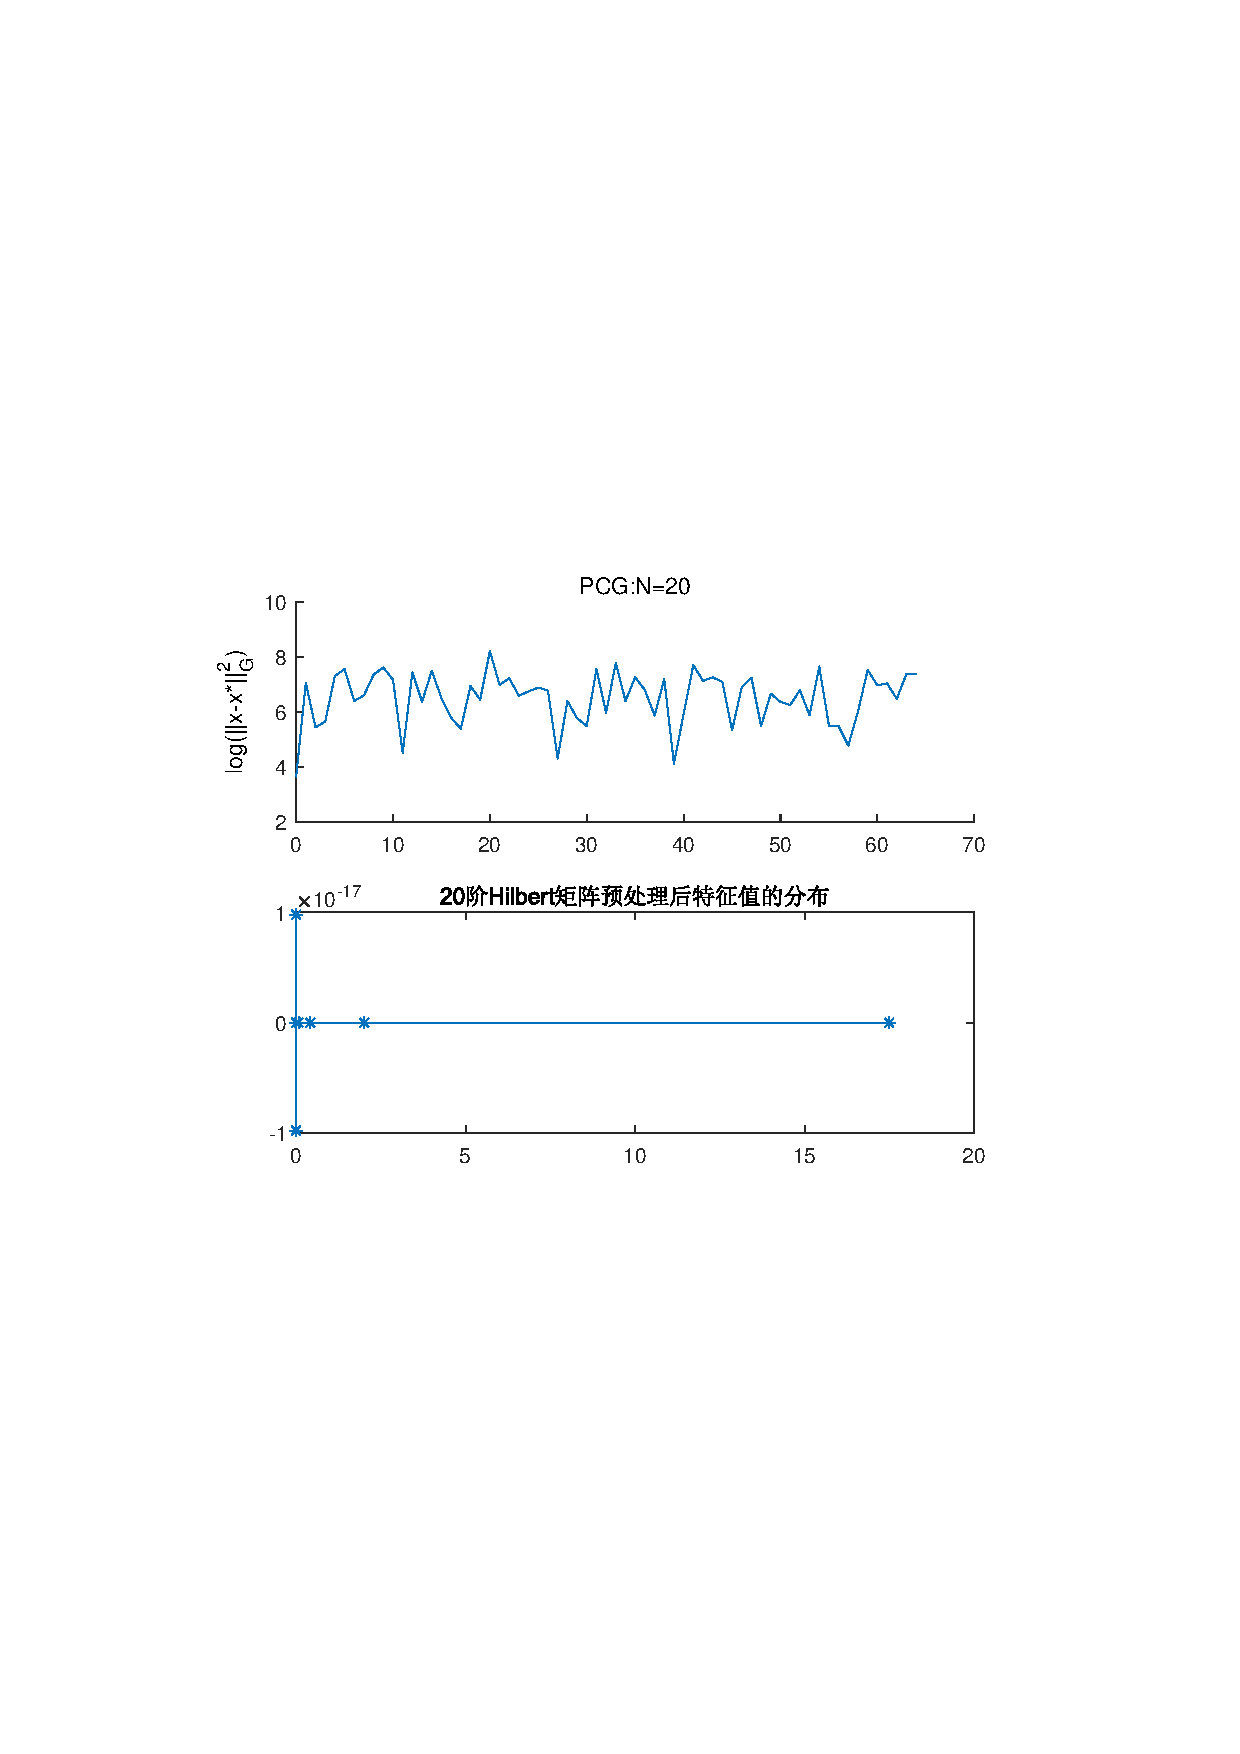
\includegraphics[width=11cm]{fig/5_7.pdf}
\end{figure}

可见这个预处理确实把特征值都聚集到一起了,但是迭代次数却为65次,仅仅比之前减少了一步,优化不太明显,这令我非常困惑,于是我改变终止精度进行测试,结果如下:

\begin{table}[htbp]
  \centering
  \caption{不同精度下迭代次数的比较$(N=20)$}
    \begin{tabular}{ccccc}
\toprule
{Error} &$10^{-6}$&$10^{-7}$& $10^{-8}$ \\
	\midrule
{Steps of CG}&66&121   & 520  \\
{Steps of PCG}&65&115   & 314 \\
\bottomrule
    \end{tabular}
\end{table}

可见在精度要求较低的情况下,两者的相差并不明显。

然后我试着将$N$调到100,观察其迭代情况,发现在精度较低时,PCG法所迭代的次数有时候甚至比CG法还要多,但在精度要求达$10^{-8}$ 时,CG法无论如何迭代都无法满足精度要求,而PCG略胜一筹,精度高出了一个数量级,且迭代次数更少。

\begin{table}[htbp]
  \centering
  \caption{不同精度下迭代次数的比较$(N=100)$}
    \begin{tabular}{ccccccc}
\toprule
{Error} &		$10^{-3}$	&		$10^{-4}$		&		$10^{-5}$		&$10^{-6}$		&		$10^{-7}$		& 	$10^{-8}$ \\
	\midrule
{Steps of CG}&12&	25&	47&175&748  & 2132(error=1.132e-08)  \\
{Steps of PCG}&15&	27&	65&111&756   & 1686(error=9.683e-09)\\
\bottomrule
    \end{tabular}
\end{table}


此外,该书上还列举了梯度下降法(PG)和预处理共轭梯度法(PCG)在求解该问题上的比较,我认为比较有借鉴意义,贴在下面:
\begin{figure}[H]
\centering
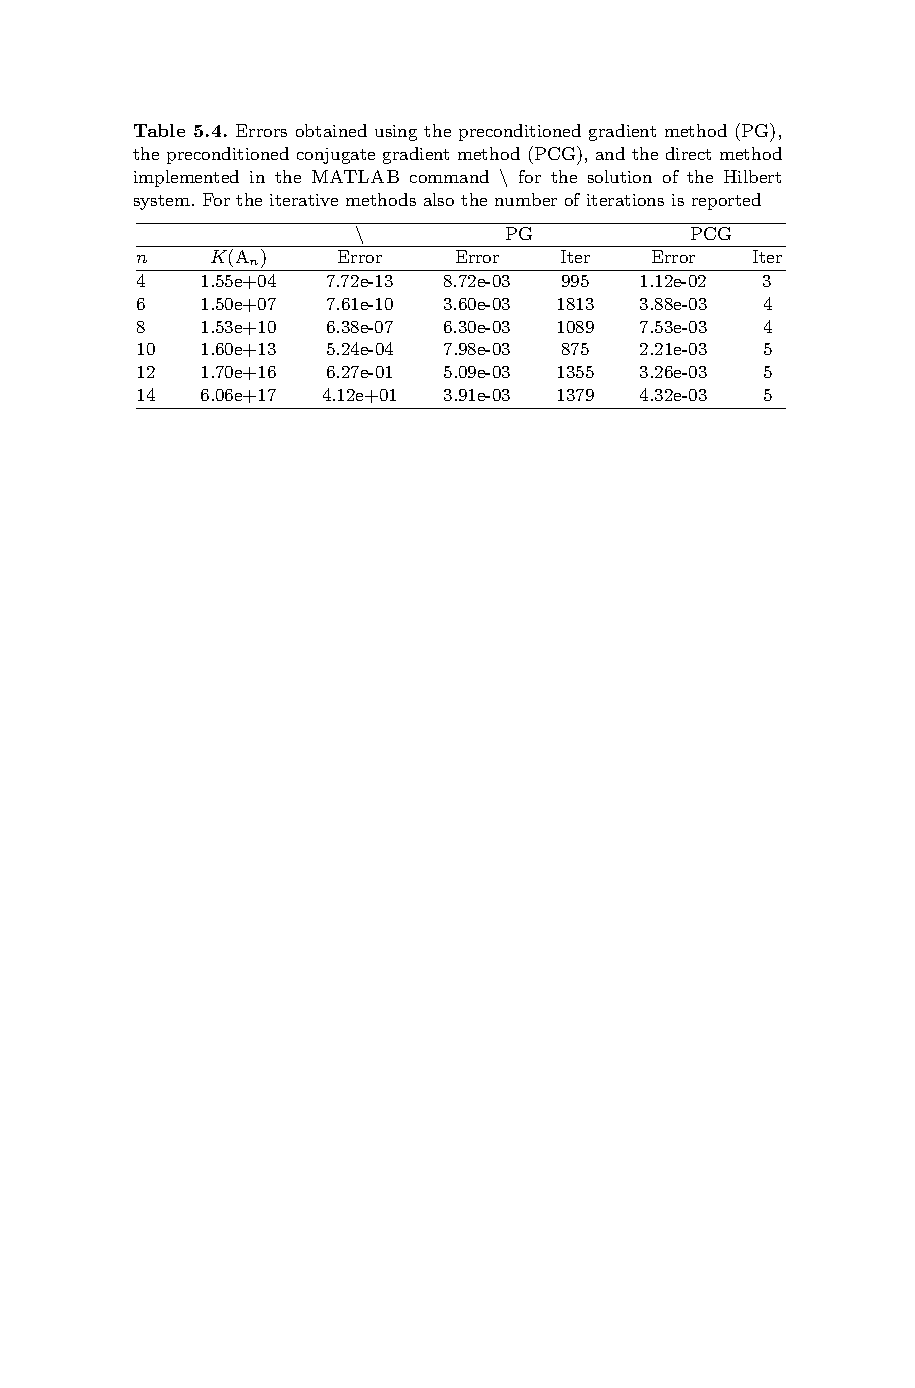
\includegraphics[width=12.5cm]{fig/5_6.pdf}
\end{figure}

$N=20$时,有/无预处理的共轭梯度法迭代情况如下:\footnote{第一个图的精度要求为$10^{-7}$,第二个图的精度要求为$10^{-8}$}
\begin{figure}[H]
\centering
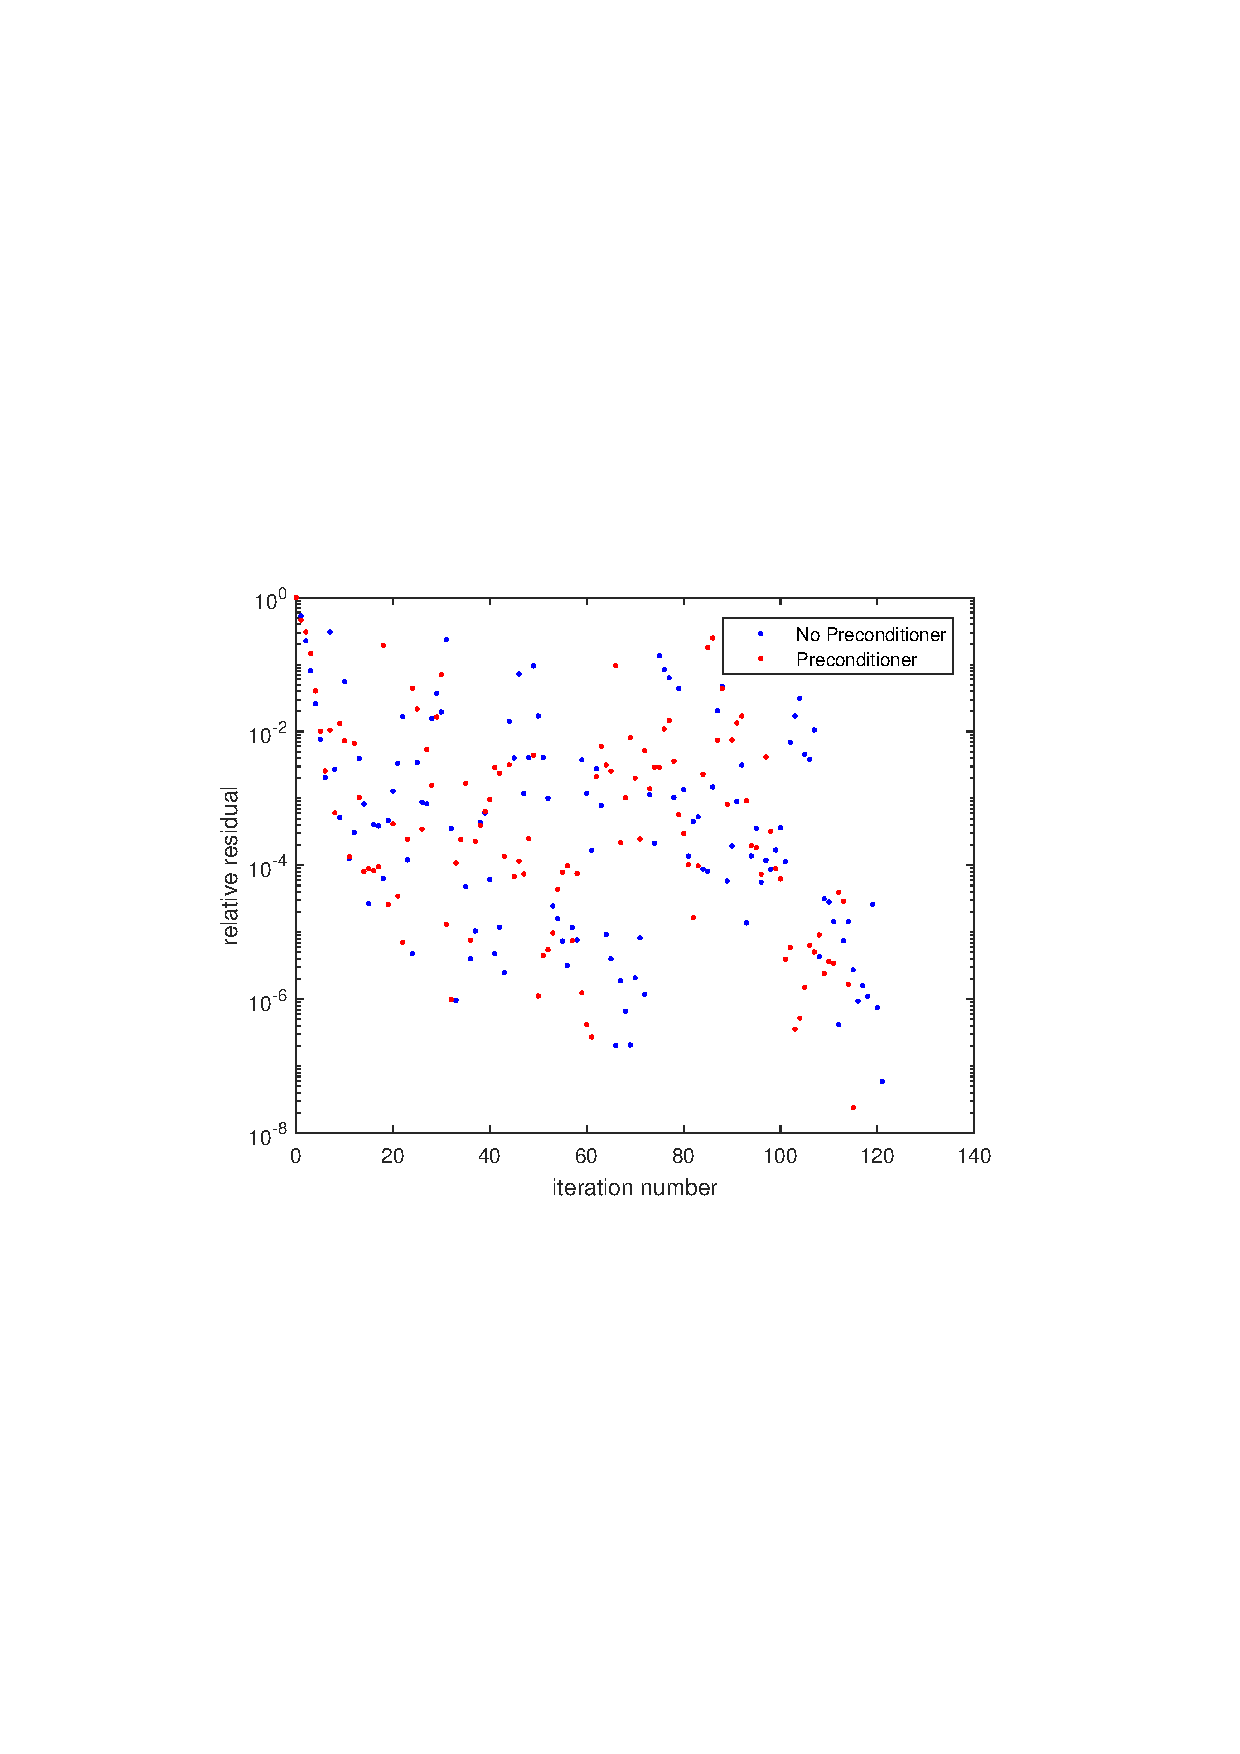
\includegraphics[width=10.8cm]{fig/5_8.pdf}
\end{figure}

\begin{figure}[H]
\centering
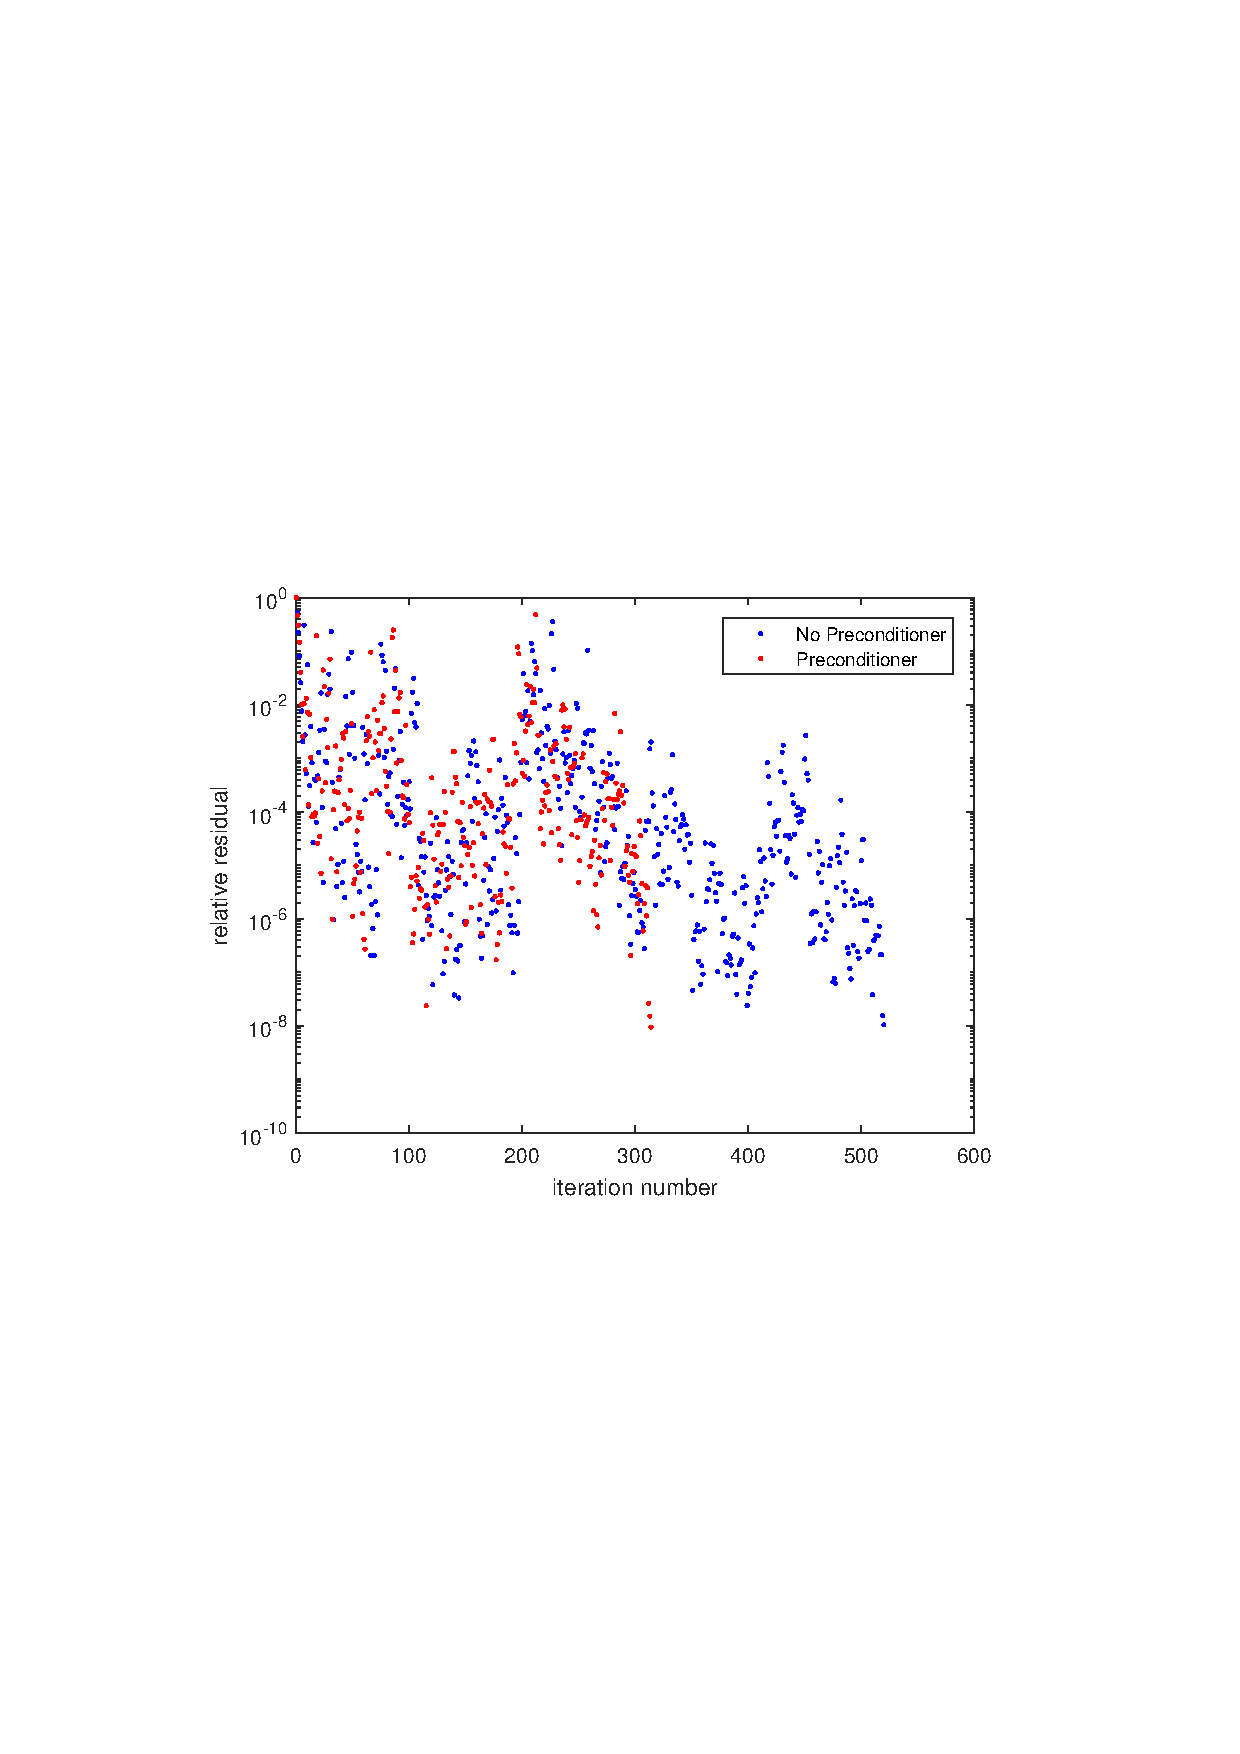
\includegraphics[width=10.8cm]{fig/5_9.pdf}
\end{figure}
